\documentclass[twoside]{article}
\usepackage{aistats2016}
\usepackage{hyperref}
\usepackage{amsmath, amssymb, amsthm, graphicx, algorithm}
\usepackage{algpseudocode}
\usepackage{caption}
%\usepackage{subcaption}
\usepackage{blkarray}
\usepackage{xcolor}
\usepackage[all,cmtip]{xy}
\usepackage{subfigure}
\usepackage[margin=0.8in]{geometry}


%\usepackage[accepted]{aistats2016}

% If your paper is accepted, change the options for the package
% aistats2016 as follows:
%
%\usepackage[accepted]{aistats2016}
%
% This option will print headings for the title of your paper and
% headings for the authors names, plus a copyright note at the end of
% the first column of the first page.

\newcommand{\A}{\mathcal{A}}
\newcommand{\C}{\mathcal{C}}
\newcommand{\D}{\mathcal{D}}
\newcommand{\G}{\mathcal{G}}
\newcommand{\B}{\mathcal{B}}
\newcommand{\E}{\mathcal{E}}
\newcommand{\cS}{\mathcal{S}}
\newcommand{\U}{\mathcal{U}}
\newcommand{\cL}{\mathcal{L}}
\newcommand{\N}{\mathcal{N}}
\newcommand{\cO}{\mathcal{O}}
\newcommand{\M}{\mathcal{M}}
\newcommand{\bN}{\mathbb{N}}
\newcommand{\bQ}{\mathbb{Q}}
\newcommand{\Exp}{\mathbb{E}}
\newcommand{\bC}{\mathbb{C}}
\newcommand{\bR}{\mathbb{R}}
\newcommand{\bZ}{\mathbb{Z}}
\newcommand{\bK}{\mathbb{K}}
\newcommand{\bF}{\mathbb{F}}

\newcommand{\fF}{\mathbf{F}}
\newcommand{\fA}{\mathbf{A}}
\newcommand{\Grp}{\mathbf{Grp}}
\newcommand{\Set}{\mathbf{Set}}
\newcommand{\Mor}{\mathrm{Mor}}
\newcommand{\Aut}{\mathrm{Aut}}
\newcommand{\Gal}{\mathrm{Gal}}
\newcommand{\Char}{\mathrm{char}}
\newcommand{\SL}{\mathrm{SL}}
\newcommand{\GL}{\mathrm{GL}}
\newcommand{\Span}{\mathrm{span}}
\newcommand{\Hom}{\mathrm{Hom}}
\newcommand{\Ext}{\mathrm{Ext}}
\newcommand{\im}{\mathrm{im}}
\newcommand{\col}{\mathrm{col}}
\newcommand{\argmax}{\mathrm{argmax}}
\newcommand{\cone}{\mathrm{cone}}
\newcommand{\rank}{\mathrm{rank}}
\newcommand{\RP}{\mathbb{R}\mathrm{P}}
\newcommand{\tr}{\mathrm{tr}}

\newcommand{\df}{\overset{\text{def}}{=}}
%\newcommand{\deg}{\mathrm{deg}}

\newcommand{\vx}{\mathbf{x}}
\newcommand{\vy}{\mathbf{y}}
\newcommand{\vu}{\mathbf{u}}
\newcommand{\vv}{\mathbf{v}}
\newcommand{\va}{\mathbf{a}}
\newcommand{\vb}{\mathbf{b}}
\newcommand{\vc}{\mathbf{c}}
\newcommand{\vd}{\mathbf{d}}
\newcommand{\vg}{\mathbf{g}}
\newcommand{\vk}{\mathbf{k}}
\newcommand{\vw}{\mathbf{w}}
\newcommand{\vz}{\mathbf{z}}
\newcommand{\vp}{\mathbf{p}}
\newcommand{\vq}{\mathbf{q}}
\newcommand{\vS}{\mathbf{S}}
\newcommand{\vf}{\mathbf{f}}
\newcommand{\bo}{\mathbf{1}}
\newcommand{\bz}{\mathbf{0}}
\newcommand{\id}{\mathrm{id}}

\theoremstyle{theorem}
\newtheorem{thm}{Theorem}

\theoremstyle{theorem}
\newtheorem{prop}{Proposition}
\theoremstyle{theorem}
\newtheorem{cor}{Corollary}

\theoremstyle{lemma}
\newtheorem{lemma}{Lemma}

\theoremstyle{definition}
\newtheorem{defn}{Definition}

\theoremstyle{example}
\newtheorem{ex}{Example}

\newcommand\undermat[2]{%
  \makebox[0pt][l]{$\smash{\underbrace{\phantom{%
    \begin{matrix}#2\end{matrix}}}_{\text{$#1$}}}$}#2}
    
\newcommand\overmat[2]{%
  \makebox[0pt][l]{$\smash{\color{black}\overbrace{\phantom{%
    \begin{matrix}#2\end{matrix}}}^{\text{\color{black}#1}}}$}#2}
\usepackage{tabularx}

\begin{document}
\input xy
\xyoption{all}
\xyoption{arc}
\makeatletter
\def\BState{\State\hskip-\ALG@thistlm}
\makeatother
% If your paper is accepted and the title of your paper is very long,
% the style will print as headings an error message. Use the following
% command to supply a shorter title of your paper so that it can be
% used as headings.
%
%\runningtitle{I use this title instead because the last one was very long}

% If your paper is accepted and the number of authors is large, the
% style will print as headings an error message. Use the following
% command to supply a shorter version of the authors names so that
% they can be used as headings (for example, use only the surnames)
%
%\runningauthor{Surname 1, Surname 2, Surname 3, ...., Surname n}

\twocolumn[

\aistatstitle{Analyzing Boston 311 Responses with Gaussian Mixture Models}

\aistatsauthor{ Jane Huang \And Isadora Nun \And Weiwei Pan \And Francisco Rivera}

\aistatsaddress{ Harvard University \And Harvard University \And Harvard University \And Harvard University} ]

\begin{abstract}
While phone calls to Boston 311 are the traditional method of reporting to city non-emergency services, requests with a smartphone app have become increasingly popular. To explore whether the app facilitates increases in the efficiency of responses to different parts of the city, and whether there are latent classes of requests, we approximate the distribution of the response times, longitude, and latitude of 311 requests with Gaussian mixture models. We compare expectation maximization and simulated annealing as methods for obtaining point estimates of the parameters, and then use Gibbs sampling to obtain the posterior distributions. We find that while app and call requests differ somewhat in service needs and geography, they break down into similar clusters along the response time axis, suggesting that users of the 311 app are overall served as efficiently as those who call. 
\end{abstract}
\section{Introduction}
In Boston, thousands of requests are made each week to city non-emergency services to address issues such as graffiti, potholes, and broken traffic signals \cite{walshpressrelease}. Requests made to non-emergency services fall under the umbrella of Boston 311.\footnote{When city non-emergency services was rebranded recently as Boston 311, the Citizens Connect App was renamed BOS:311. We refer to the app as Citizens Connect throughout for continuity.} Ensuring that requests are fulfilled in a timely manner and that services are accessible to all segments of the population is essential for maintaining the safety and well-being of city residents. 

Traditionally, requests for city non-emergency services have been made through phone calls, but as smartphone technology became increasingly common, the Citizens Connect app was introduced in 2009 to allow Boston residents to report problems to 311 through a mobile phone interface \cite{newurbanmechanics}. The app developers state their motivation as: ``Residents report public issues directly from their smart phones into the City's work order management system so that it gets immediately to the right person in City Hall to fix the problem...We were interested in seeing if we could engage more or different residents" \cite{newurbanmechanics}.  

To assess the extent to which the 311 app can help to deliver efficient responses to areas that may be comparatively underserved through the traditional mode of non-emergency service requests, we seek to model the joint distribution of response times and locations for 311 requests. Using our model, we aim to compare the distributions of requests originating from constituent calls and those made via the mobile phone app. Because we are interested in identifying whether there are hidden sub-populations of requests that are distinguishable by the observed locations and response times, we use Gaussian mixture models to approximate the distributions. 
\section{Data}
Records of Boston's 311 service requests were obtained from \url{https://data.cityofboston.gov/City-Services/311-Service-Requests/awu8-dc52}. We first selected, from all closed complaints, requests that had been opened in 2015 through either constituent calls or the Citizens Connect App. The descriptors extracted for the data included the times that the complaints were opened and closed by the city (reported to the nearest second) and the longitude and latitude of the source of the complaint. A new variable, response time, was defined as the difference between the reported closing and opening times of a 311 complaint. Because the numerical scale of response times is much larger than those of longitude and latitude, the values for each variable were rescaled to have zero mean and unit variance. The mean response time is 13.2 days with standard deviation 29.1 days. The mean latitude is 42.326 with standard deviation 0.034. The mean longitude is -71.083 with standard deviation 0.035. The data were subsequently split apart into two sets based on origin of request (constituent calls or the Citizens Connect App). 

Since the dataset is very large, a randomly selected subsample was used for the analysis to reduce computational expense. For the expectation maximization estimates, the data were down-sampled to provide $\sim20,000$ points each for constituent call and the Citizens Connect App analysis. For Gibbs sampling, the data were down-sampled to provide $\sim10,000$ points for each group. Subsamples of this size still provide good coverage across the city. 
\section{Methods}
\subsection{Bayesian Gaussian Mixture Models}
\begin{figure}
\begin{center}
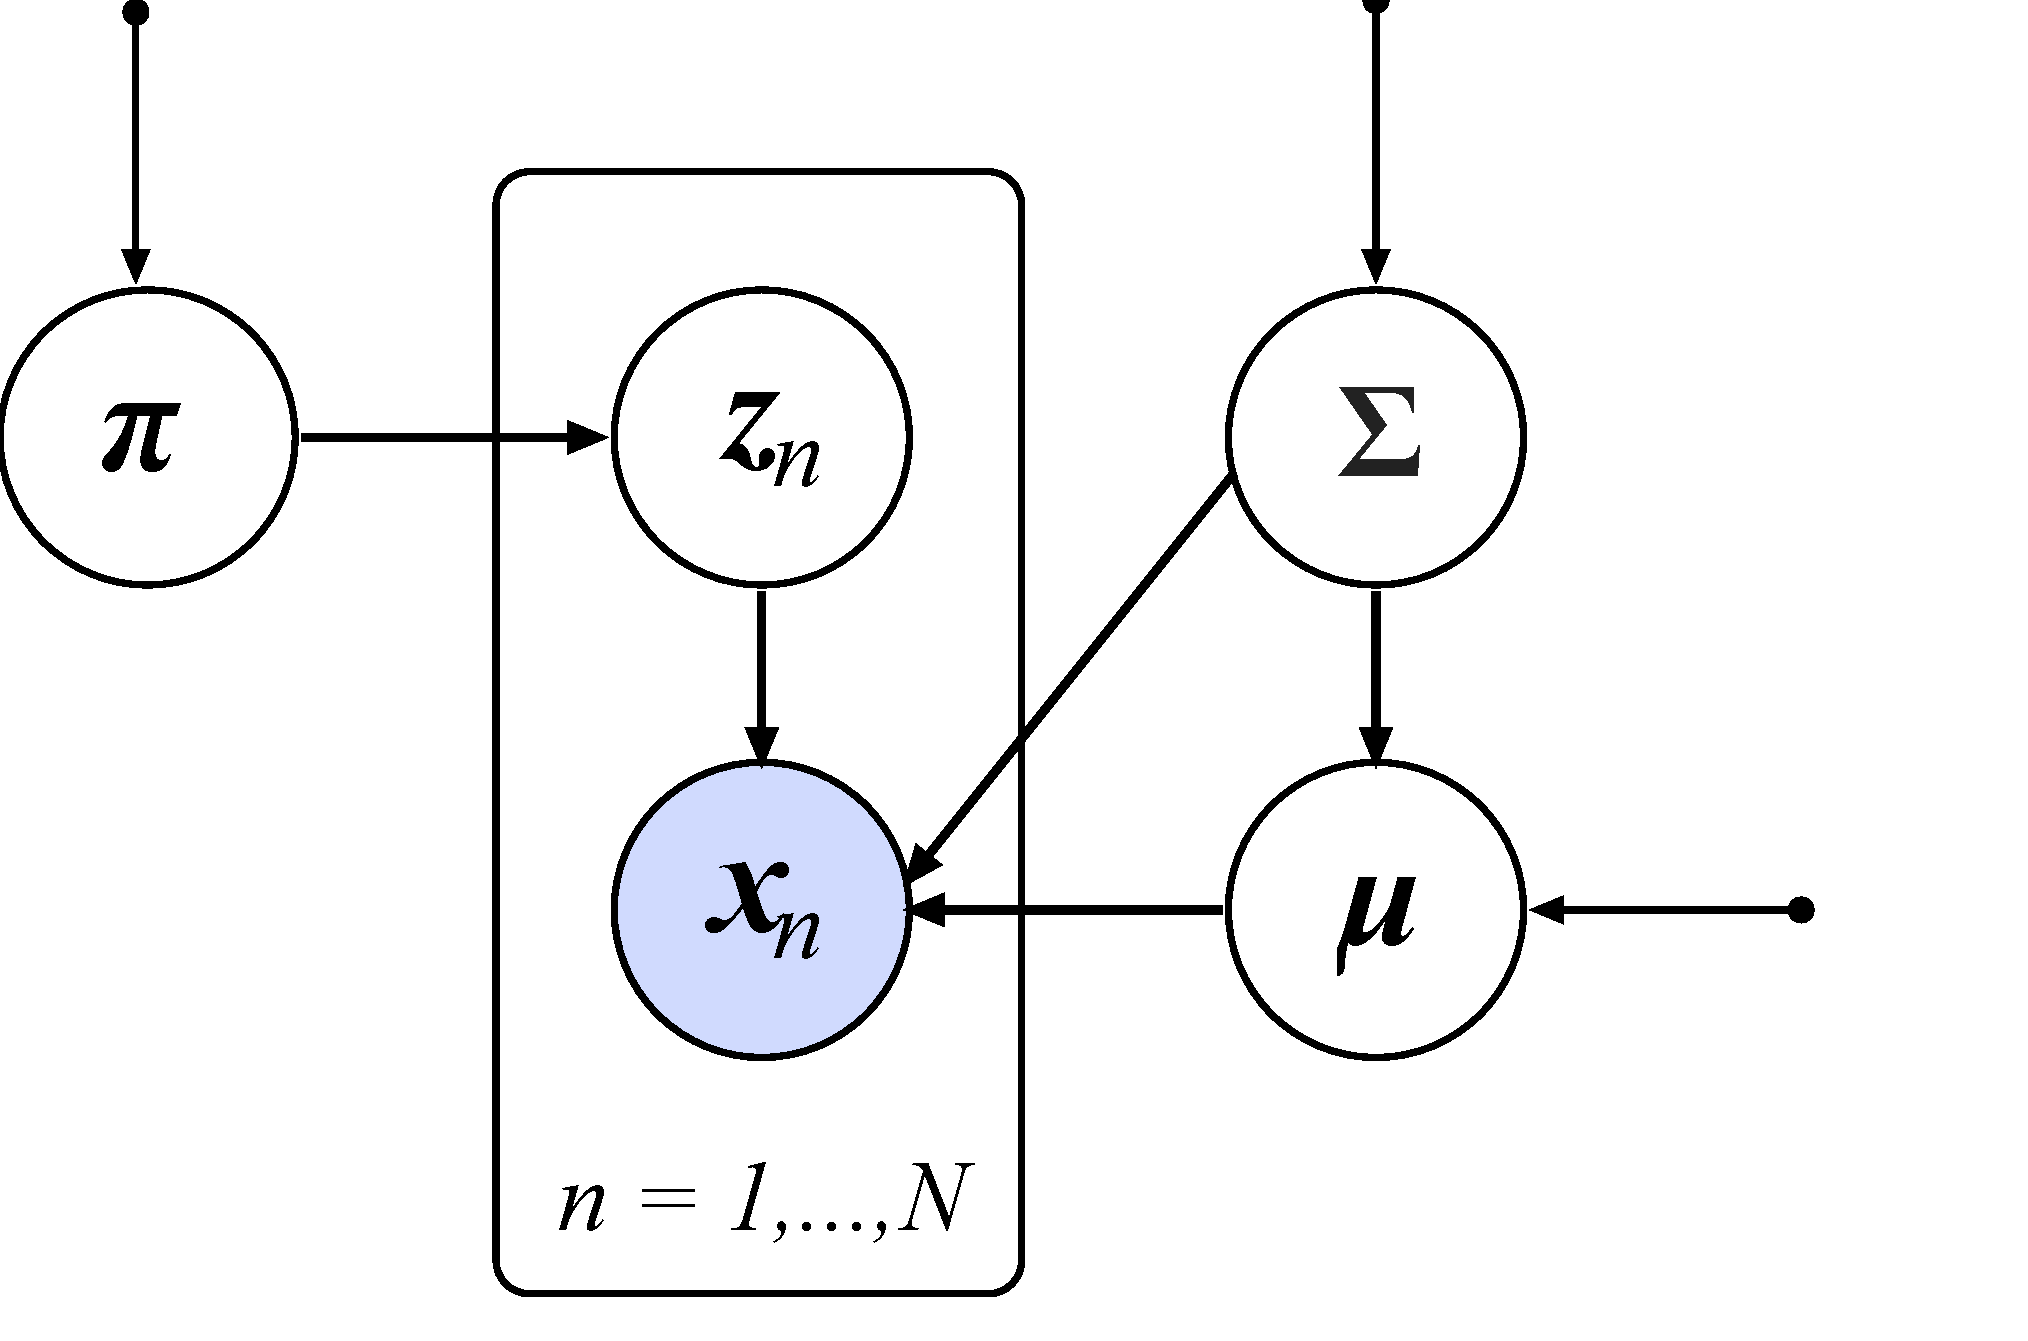
\includegraphics[width=50mm]{graph_model}
\caption{Diagram of Gaussian mixture model}
\end{center}
\end{figure}
Each 311 request is described by a three-dimensional vector consisting 
\begin{align}
x_n = (\text{response time, longitude, latitude}). 
\end{align}
We model the distribution of these data points as a mixture of $K$ Gaussian components with means $\mu = \{\mu_k :  1\leq k\leq K\}$ and covariance matrices $\Sigma = \{\Sigma_k :  1\leq k\leq K\}$. The mixture coefficients for the model (i.e., the fraction of the population belonging to each component) are represented by $\pi$, a vector with $K$ elements.  

Since the component membership is not known, we specify the component membership indicators as $\mathbf{Z} = (z_1, \ldots, z_N)$. Each indicator for datapoint $x_n$ is a $K$-element vector $z_n$, defined such that \begin{align}
z_{nk} = \begin{cases}
1, & x_n\text{ belongs to the $k$-th component}\\
0, & \text{otherwise}. 
\end{cases}
\end{align}
Hence, the complete data likelihood is 
\begin{align}
L(\mathbf{X}) = \prod_{n=1}^N\prod_{k=1}^K \N(x_n| \mu_k, \Sigma_k)^{z_{nk}}.
\end{align}
The prior for $\pi$ is a Dirichlet distribution, which is appropriate for generating vectors that sum to 1. For $\Sigma$, we use an Inverse-Wishart prior, which is conjugate to the multivariate normal distribution and ensures the selection of a positive-definite matrix, as required for a covariance matrix. The hyper-parameters for the Inverse-Wishart prior are the scale matrix $S_0$ and the degrees of freedom $\nu_0$.  These priors can be set to be weakly informative, which is useful because it is difficult to assess \textit{a priori} what the components in the 311 data should be. In addition, while the posterior does not have a closed form, these priors allow closed forms of the conditional distributions to be used in Gibbs sampling to explore the posterior distribution. 

To summarize, our model is described by the following (as adopted from \cite{Gelman, Jones}): 
\begin{align}
\pi &\sim Dir(\alpha_0)\\
\Sigma_k &\sim \mathrm{IW}(S_0, \nu_0)\\
\mu_k | \Sigma_k &\sim \N(m_0, V_0)\\
z_n | \pi &\sim \prod_{k=1}^K \pi_k^{z_{nk}}\\
x_n | \mathbf{Z}, \mu, \Sigma &\sim \prod_{k=1}^K \N(\mu_k, \Sigma_k)^{z_{nk}}
\end{align}

\subsection{MAP computation and model selection}
Expectation maximization (EM) was used to compute point estimates via both maximum likelihood estimates (MLE) and maximum a posteriori estimates (MAP). EM is particularly appropriate for models with missing labels. The computation for MLE was initialized with the parameters $\mu$, $\pi$, $\Sigma$ using the means, mixture coefficients and covariance matrices for the components obtained from K-means clustering. The EM algorithm update equations for MLE are as follows \cite{Bishop}: 

For the E-step, we calculate   
\begin{align}
r_{nk} = \frac{\pi_k p\left(\mathbf{x}_n | \mu_k, \Sigma_k\right)}{\sum_{k'=1}^K \pi_{k'} p\left(\mathbf{x}_n | \mu_{k'}, \Sigma_{k'}\right)}
\end{align}

which expresses the probability that $z_{nk}=1$ given the observations. These probabilities are used as weights in the M-step to calculate new values of $\mu$, $\Sigma$, and $\pi$:
\begin{align}
\pi_k &= \frac{r_k}{N},\;\; r_k =\sum_{n=1}^N r_{nk}\\
\mu_k &=\frac{\sum_{n=1}^N r_{nk}\mathbf{x}_n}{r_k}\\
\Sigma_k &= \frac{\sum_{n=1}^N r_{nk} \mathbf{x}_n\mathbf{x}_n^\top}{r_k} - \mu_k\mu_k^\top
\end{align}
The MLE values for the parameters $\mu$, $\pi$ and $\Sigma$ were used to initialize EM for computing MAP estimates of the parameter. While the E-step in the MAP computation is the same as that for MLE, the updates in the M-step incorporate the model priors (update equations as given in \cite{Bishop}). For example, the step to update $\pi$ is now 
\begin{equation} 
\pi_k = \frac{r_k + \alpha_k - 1}{N + \sum_{k=1}^K \alpha_k - K},
\end{equation}
where $\alpha$ is the shape parameter for the Dirichlet prior for $\pi$. 
For analysis of component characteristics, MAP estimates of the parameters are used, since MLE tend to overfit the data even with model selection. 
\begin{figure}[h!]
\begin{center}
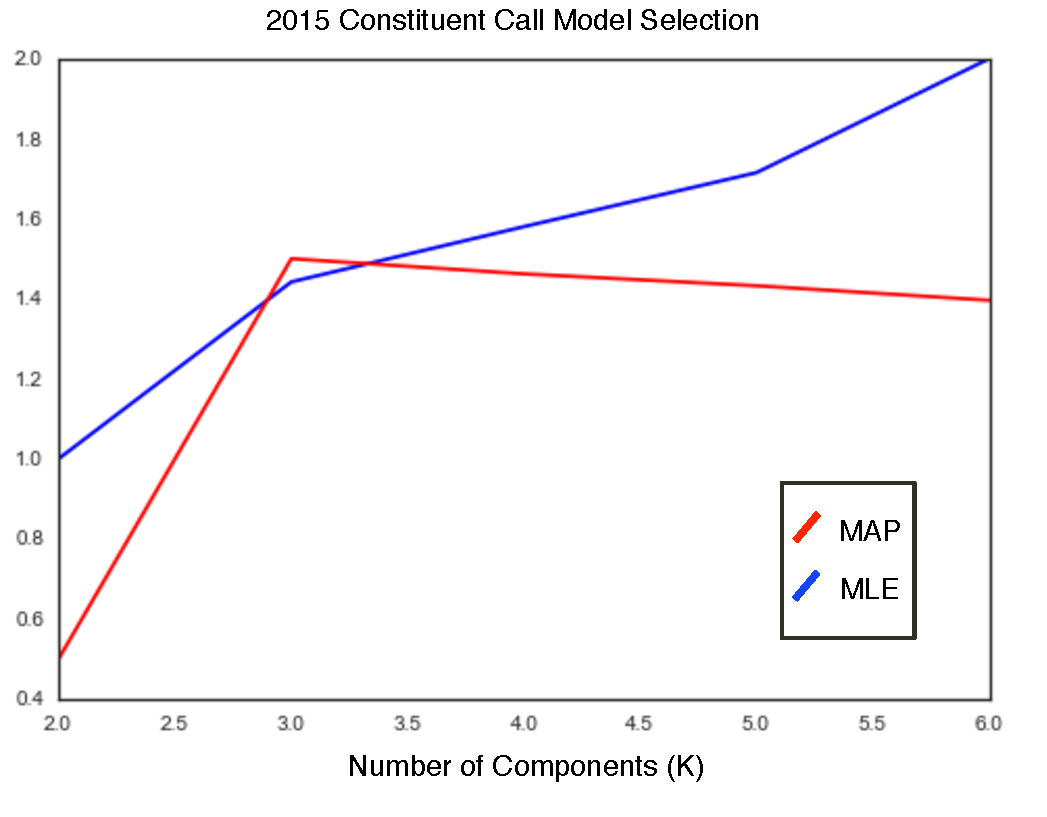
\includegraphics[width=60mm]{Call_bic}
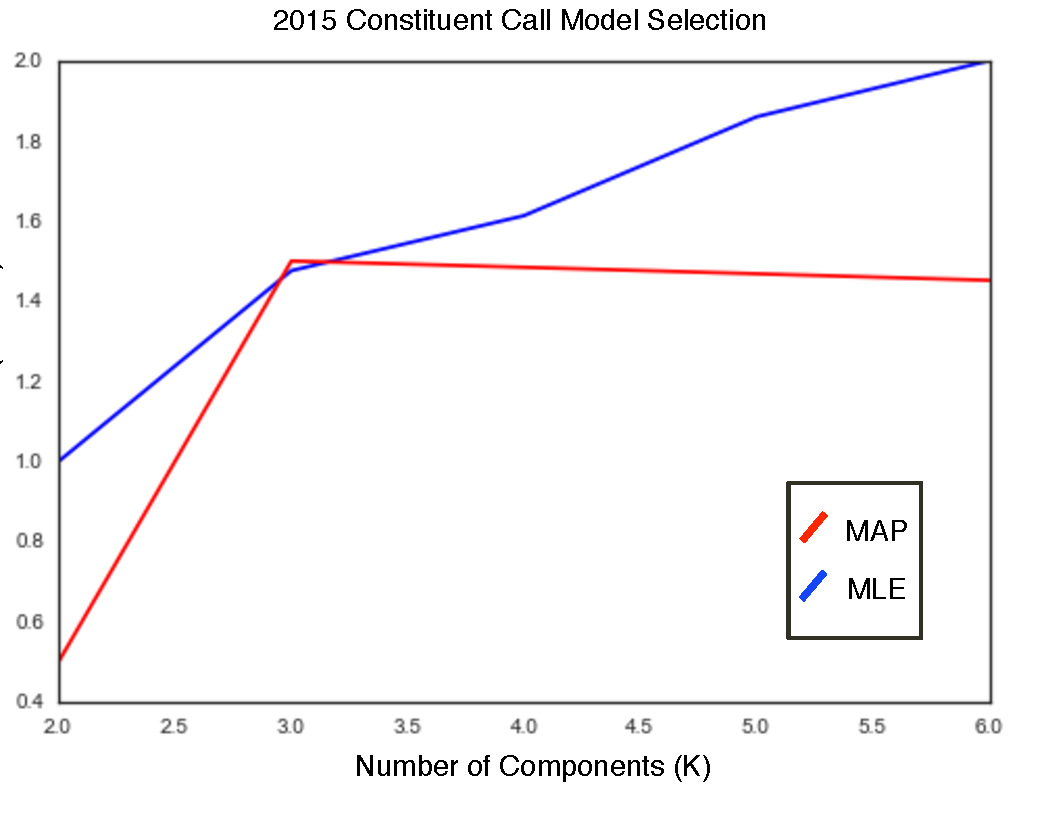
\includegraphics[width=60mm]{App_bic}
\caption{Model Selection Using BIC Scores (Scaled)}\label{fig:bic}
\end{center}
\vskip -0.2in
\end{figure} 

We performed model selection for the optimal number of components, $K$, using the Bayesian Information Criterion (BIC). The BIC score is an approximation for the evidence for the data $\log p(X | \mathcal{M})$ given the model $\mathcal{M}$, assuming the data distribution belongs to the exponential family \cite{Bishop}. Using maximum likelihood estimators, it is defined as 
\begin{equation}
\mathrm{BIC} = \log\mathcal{L}(\mathbf{X} | \theta^{MLE}, \mathcal{M}) - \frac{1}{2} \kappa_\mathcal{M}  \log(N),
\end{equation}
where $\mathcal{L}$ is the likelihood of the data, $X$, given the model, $\mathcal{M}$, and the maximum likelihood parameters of the model, $\theta^{MLE}$; $\kappa_\mathcal{M}$ is the number of free parameters in $\mathcal{M}$ and $N$ is the size of the data. Higher BIC scores indicate that a model is a better fit for the data without overfitting. In a Bayesian framework, we want to select the model with the largest posterior probability, which involves choosing the model with the largest integrated complete likelihood (ICL). A BIC-like approximation of the ICL proposed by Biernacki et al. \cite{Biernacki} is: 
\begin{align}
\mathrm{BIC} = \log \mathcal{L}(\mathbf{X}, \mathbf{Z} | \theta^{MAP},  \mathcal{M}) -  \frac{1}{2} \kappa_\mathcal{M} \log(N),
\end{align}
where $X$ is the data, $\theta^{MAP}$ are parameters estimated from the posterior modes and $Z$ represents the latent cluster labels. 

We computed both MLE and MAP estimates for different models with $K=2$ to $K=6$ number of components. The BIC scores were then computed for each model given these estimates. From Figure \ref{fig:bic}, the BIC scores indicate that $K = 3$ is the optimal number of components for fitting our model using MAP estimates. Note also, from Figure \ref{fig:bic}, that MLE continues to favor models with larger numbers of components even after penalizing model complexity. Thus, MLE will tend to overfit the data.

\subsection{Simulated Annealing}
As an alternative to EM for computing the maximum likelihood estimates of our model parameters, we considered likelihood maximization via simulated annealing.  Our state space consists of the mean vectors and covariance matrices for each clusters, and the objective function is the negative log-likelihood of observing the data given the present parameters. We minimize the objective function to find the maximum likelihood parameters.

One important implementation decision is how to jump to a new state. For a cluster with mean $\mu$ and covariance matrix $\Sigma$, a jump must propose a new mean and covariance. To find the proposed mean, we take the present estimate of the mean and add Gaussian noise distributed with a covariance matrix proportional to that of the cluster. In other words,
$$\mu_\text{proposed} \sim \mathcal{N}(\mu, c\Sigma)$$
where $c$ is tuned for optimal performance. For the cluster covariance matrix, we also add Gaussian noise with adjustable variance. However, since this noise may create an invalid covariance matrix, we must process the matrix to ensure that it remains symmetric and positive semi-definite by only modifying negative eigenvalues with some small positive $\epsilon$ and keeping the eigenvectors as unchanged as possible.

\subsection{Gibbs sampling of the posterior distribution}
We implemented a Gibbs sampler for the posterior distribution, since the full conditionals can be explicitly computed for our model, facilitating sampling.  The conditional distributions for our model are found in \cite{Gelman, Jones}. 

 Each iteration of the Gibbs sampler consists of the following steps: 
 \begin{enumerate}
\item The indicator variable $Z_n$ for the data point $x_n$ is drawn from a multinomial distribution with the event probabilities given by 
\begin{equation}
p(z_{nk} = 1| x_n, \mu, \Sigma, \pi)  \propto \pi_k \mathcal{N}(x_n | \mu_k, \Sigma_k)\end{equation}

\item The mixture coefficients are drawn from the conditional distribution 
\begin{equation}
p(\pi|\mathbf{Z}) = \mathrm{Dir}(\{\alpha_{0,k}+ N_k\} )
\end{equation}
where $N_k$ is the number of observations assigned to each cluster. 

\item The component means are drawn from the conditional distribution 
\begin{equation}
p(\mu_k | \Sigma_k, \mathbf{Z}, \mathbf{X}) = \mathcal{N}(\mu_k | m_k, V_k)
\end{equation}
where 
\begin{equation}
V_k^{-1} = V_0^{-1} + N_k\Sigma_k^{-1}
\end{equation}
and 
\begin{equation}
 m_k = V_k(\Sigma_k^{-1}N_k\overline{x}_k + V_0^{-1}m_0)
 \end{equation}
 with $\overline{x}_k$  defined as the mean value of the observations assigned to component $k$. 
 
\item Finally, the component covariance matrices are drawn from the conditional distribution 
 
 \begin{equation}
 p(\Sigma_k | \mu_k, \mathbf{Z}, \mathbf{X}) = IW(\Sigma_k | S_k, \nu_0+N_k)
 \end{equation}
 where 
 \begin{equation}
S_k = S_0 + \sum_{n=1}^N z_{nk}(x_n - \mu_k)(x_n - \mu_k)^\top
\end{equation}

\end{enumerate}

A common issue arising from sampling from Gaussian mixture models is the ``label-switching problem." In these mixture models, the components cannot be labeled unambiguously because the likelihood remains constant when component labels are permuted.  As a result, the posterior distribution for a Gaussian mixture model may be highly multimodal, potentially leading to slow mixing of the Gibbs sampler. To address this issue, we implemented the suggestion of Gelman et al. \cite{Gelman} to resolve the labeling ambiguity of the components by defining an ordering of the mixture coefficients, $\pi_1 > \pi_2 > \pi_3$. We note that, in general, this type of identifiability constraint may not always break symmetry as desired, particularly if the fractions are similar in size \cite{Stephens}. However, based on the point estimates obtained with EM and simulated annealing, our clusters appear to be substantially different in size. Thus, imposing an order on the mixture coefficients should collapse the multimodality of our posterior distribution.

We used the MAP estimate obtained from expectation maximization to initialize the values of $\pi$, $\mu$, and $\Sigma$ for the Gibbs sampler. We then set $\alpha_0 = (1,1,1)$, $m_0 = (1,1,1)$, $\nu_0 = 3$ (the number of components in the mixture model), and $S_0$ and $V_0$ to the identity matrices to maintain weakly informative priors.   

\section{Results}

\subsection{Expectation maximization}

Expectation maximization for MAP estimation (as well as for MLE) typically converged within about 30 iterations, based on examination of the log-likelihood plotted against iteration number. The hard clustering of the data based on MAP estimations of the mixture parameters for $K=3$ are shown in Figure \ref{EMlabels}. For both Citizens Connect and call data, the identified Gaussian components are largely distinguished by differences in response time, but not by geography. For each, the largest component (85\%) has a mean response time of 4.5 days, the next largest (14\%) has a mean of 50 days, and the last lags substantially with a mean of 266 days (1\%). However, while the slow requests seem to be distributed throughout Boston for constituent calls, the slow requests are more concentrated in the downtown area for the Citizens Connect App, where request volume is high.
\begin{figure}[h!]
\begin{center}
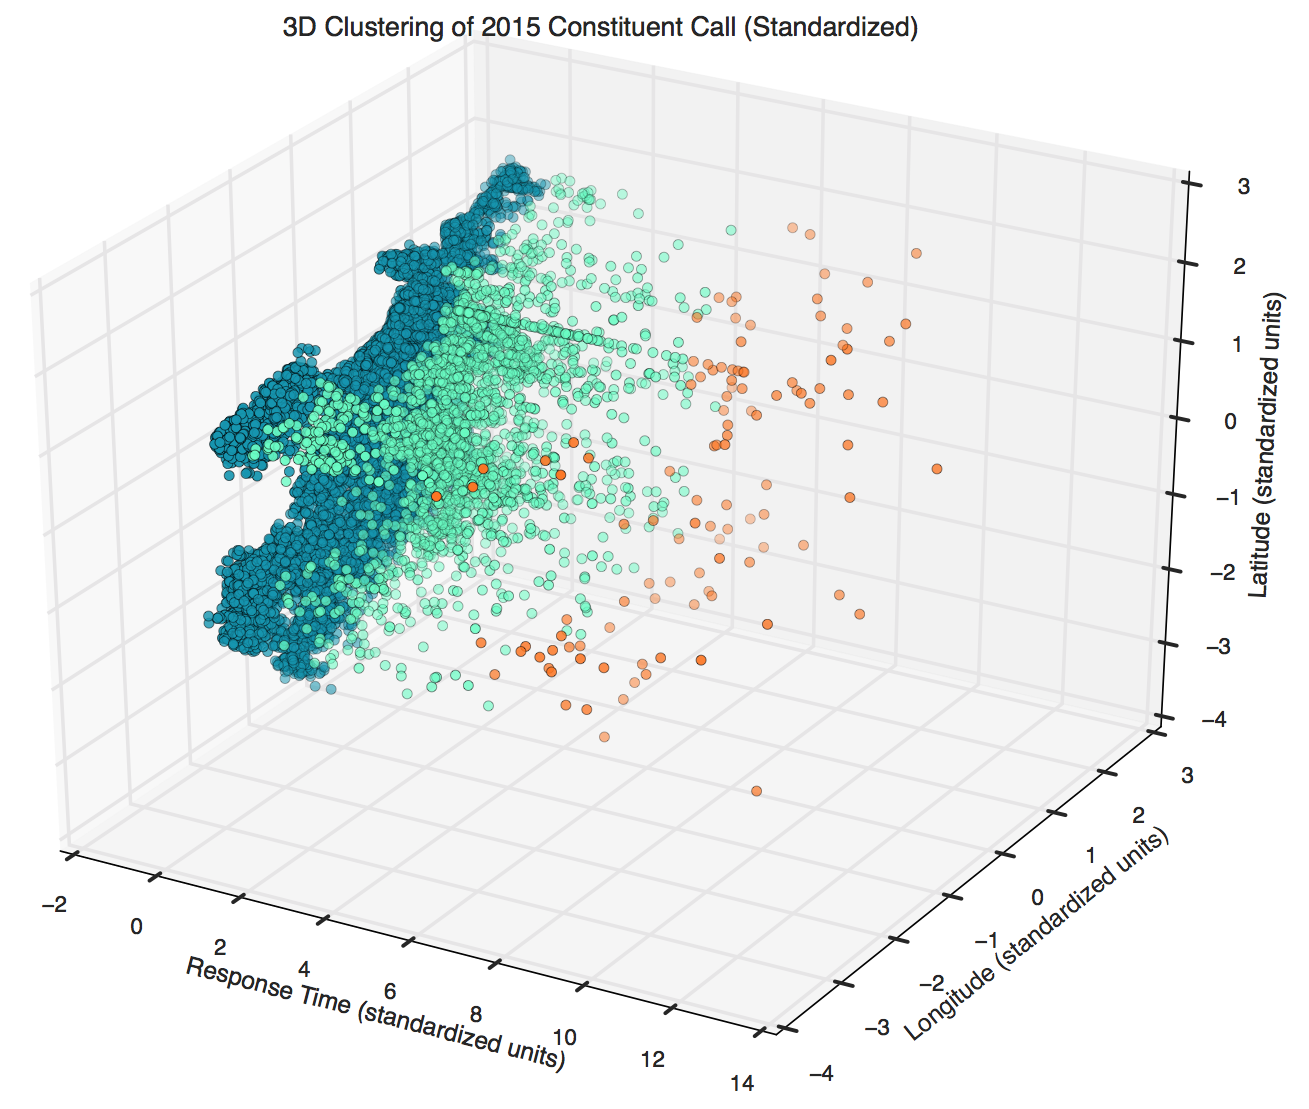
\includegraphics[width=60mm, height=50mm]{3D_call}
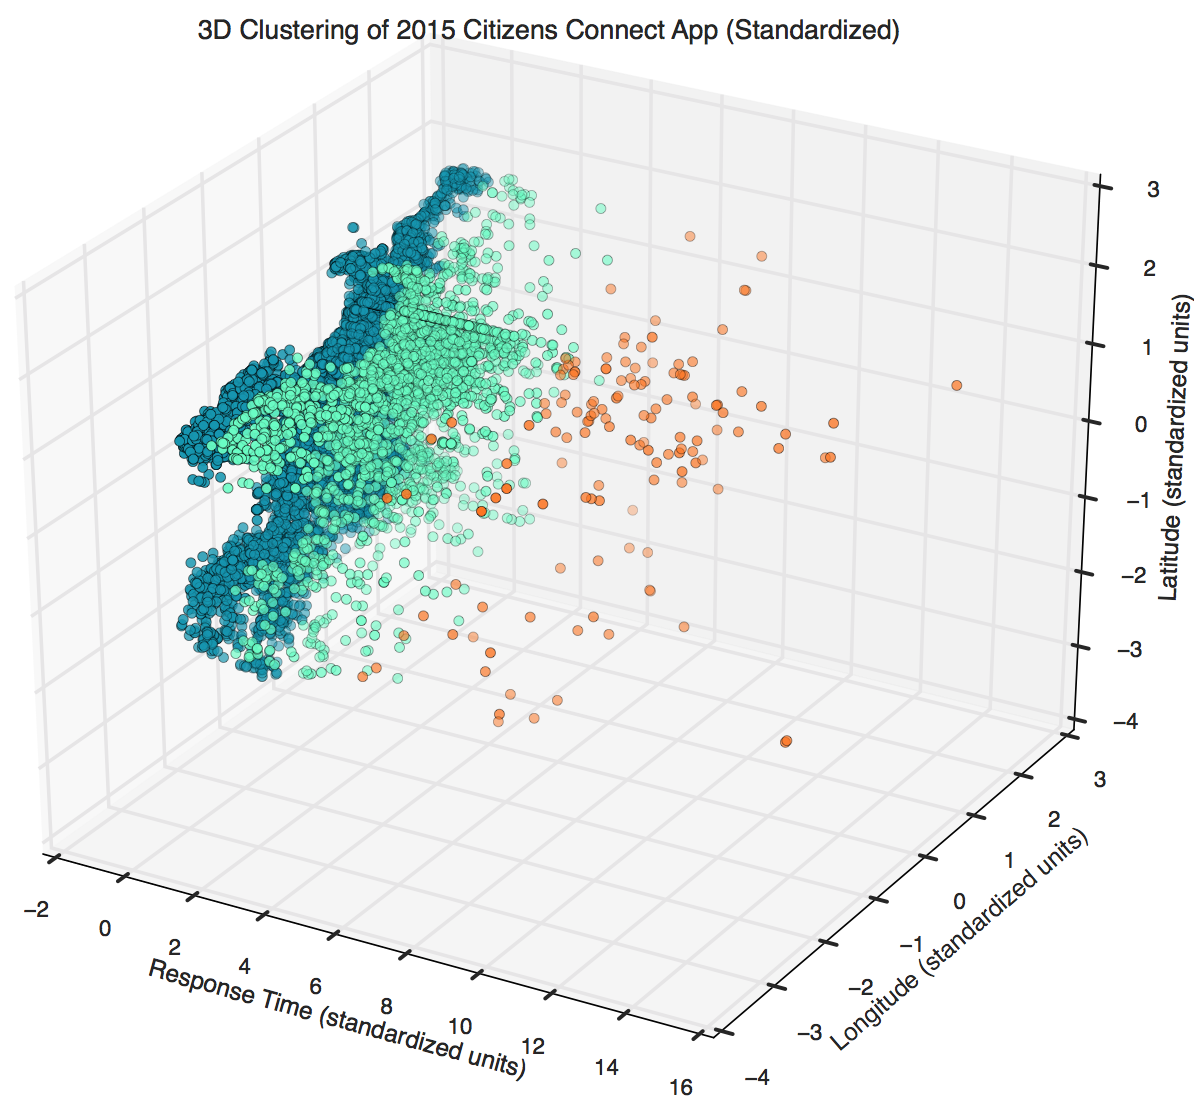
\includegraphics[width=60mm, height=50mm]{3D_app}
\caption{EM MAP label assignments}
\label{EMlabels}
\end{center}
\end{figure}

\subsection{Simulated annealing}
Simulated annealing for a 3-component model requires about 1000 iterations to converge (based on changes in the calculated likelihood), and takes longer to run even when using a smaller sub-sample (3000 observations) of the dataset compared to EM. As a point estimate method for a Gaussian mixture model, EM appears to be more efficient. Like EM, simulated annealing finds the requests dominated by a large cluster characterized by short response times, and a small cluster with lagging response times, with little geographic distinction between components. 

\begin{figure}[h!]
\begin{center}\label{SAcluster}
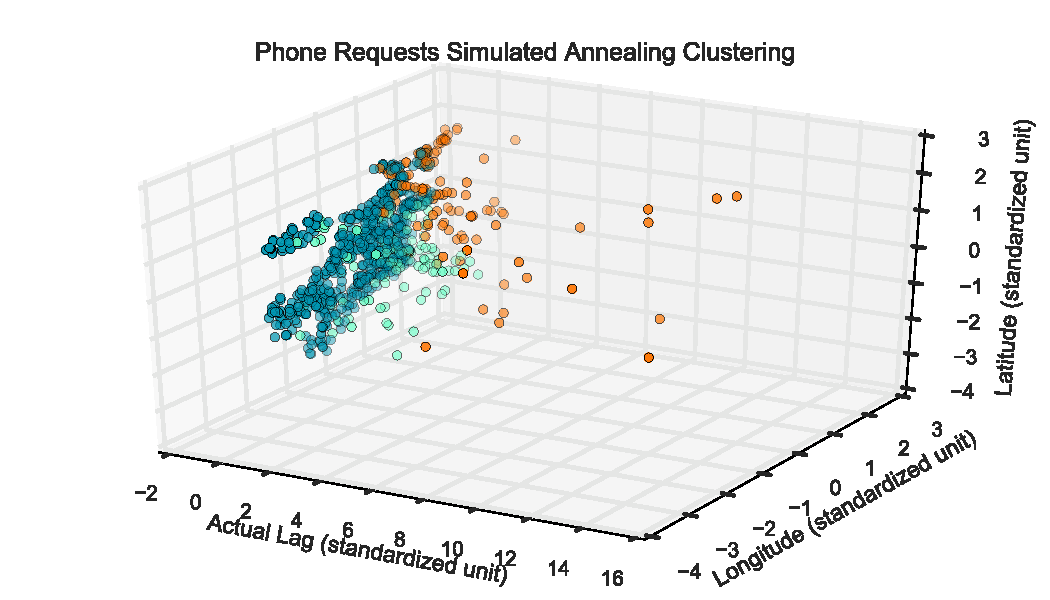
\includegraphics[width=70mm]{simulated_annealing_clustering}
\caption{Cluster assignments for call data based on simulated annealing}
\end{center}
\end{figure}


\subsection{Gibbs sampling}

\begin{table*}
\label{comparison}
\begin{center}
\begin{tabularx}{\textwidth}{c| l | l}
%\multicolumn{1}{c}{\bf PART}  &\multicolumn{1}{c}{\bf DESCRIPTION} \\
Parameter & Constituent Call & App data\\[5pt]
\hline
$\pi$ &
$\small\left(\begin{array}{@{} ccc@{} } .484\pm.006 & .328\pm.006  &.189\pm.005 \end{array}\right)$ 
&
$\small\left(\begin{array}{@{} ccc@{} } .480\pm.006 & .307\pm.006  &.213\pm.005 \end{array}\right)$\\[5pt] 
$\mu_1 $ &       
 $\small\left(\begin{array}{@{} ccc@{} } 1.04\pm.03 & -71.08768\pm .0005  &42.3221 \pm .0006 \end{array}\right)$   
&
$\small\left(\begin{array}{@{} ccc@{} } .44\pm.01 & -71.0768\pm .0006  &42.3401\pm .0005 \end{array}\right)$
\\[5pt]
$\mu_2 $        &
$\small\left(\begin{array}{@{} ccc@{} } 8.7\pm.2 & -71.0772\pm.0008  &42.3196\pm .0008 \end{array}\right)$  
&
$\left(\begin{array}{@{} ccc@{} } 6.4\pm.1 & -71.0796\pm.0009  &42.3320\pm .0009 \end{array}\right)$
\\[5pt]
$\mu_3$ &
$\small\left(\begin{array}{@{} ccc@{} } 52.5\pm1.2 & -71.0891\pm .0009  &42.3262\pm .0007 \end{array}\right)$

&
$\small\left(\begin{array}{@{} ccc@{} } 50.1\pm1.3 & -71.0856\pm .0009  &42.3379\pm .0007 \end{array}\right)$
 \\
\end{tabularx}
\vspace{1pt}
\caption{Gibbs estimates for $\pi$ and $\mu$. $\mu$ vector listed in order of (response time, longitude, latitude) in units of days and decimal degrees. Means and uncertainties for covariance matrices from Gibbs sampling are listed in the IPython notebooks due to space constraints here.}
\end{center}
\end{table*}


The Gibbs sampler ran for a total of 500 iterations for both the constituent call and app data. Inspection of the trace plots suggest that convergence was achieved after 150 iterations (see Figure \ref{trace} for sample trace plots), so a burn-in of 150 iterations was applied for calculation of the posterior means and uncertainties, listed in Table 1. (A test of a PyMC implementation of a Gaussian mixture model did not converge after 40,000 iterations, so PyMC was deemed not optimal for this problem). 

The clustering of the data based on posterior mean estimates obtained from the Gibbs sampler is shown in Figure \ref{gibbsclusters}. Compared to the MAP estimates made with EM, the Gibbs sampler characterizes the data with somewhat different components, and the results more closely resemble the MLE estimates made with EM. In particular, the Gibbs sampler results tend to assign more points to the cluster with the slowest response times and fewer to the cluster with the fastest. However, like the EM MAP estimates, the clusters with shorter response times account for larger fractions of the population, and the clusters are largely distinguished along the response time axis, with typically low covariance between response time and the location variables. 

One possible reason for the difference between the EM MAP and Gibbs sampling results is that the posterior is multimodal. In general, determining the presence of multiple modes is challenging because convergence may appear to have been achieved when in fact the sampler is only traveling around a single mode. MCMC techniques optimized for sampling multimodal distributions, such as parallel tempering or nested sampling, may be useful for exploring this issue further. 

\begin{figure}[h!]
\begin{center}
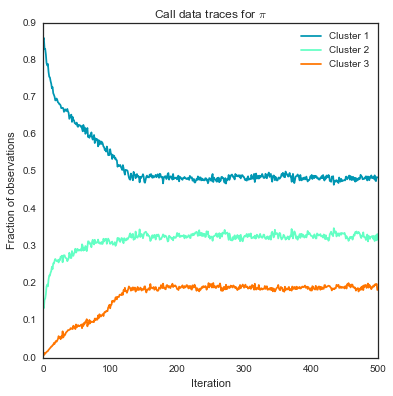
\includegraphics[width=60mm]{calldatapitrace}
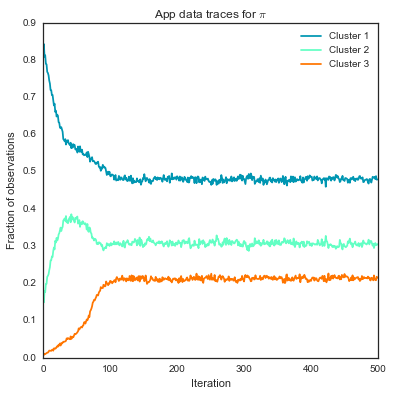
\includegraphics[width=60mm]{appdatapitrace}
\caption{Gibbs sampler traces for the $\pi$ parameter}
\label{trace}
\end{center}
\end{figure}


\begin{figure}[h!]
\begin{center}
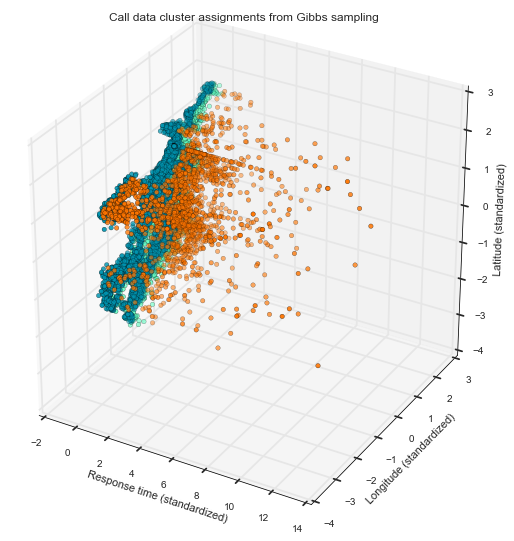
\includegraphics[width=45mm, height=42mm]{gibbscallclusterassignments}
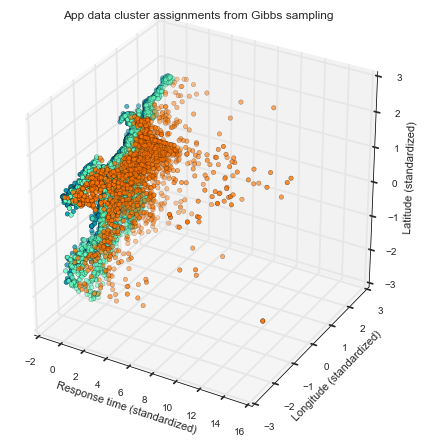
\includegraphics[width=45mm, height=42mm]{gibbsappclusterassignments}
\caption{Gibbs component assignments}
\label{gibbsclusters}
\end{center}
\end{figure}

\begin{figure}[h!]
\begin{center}
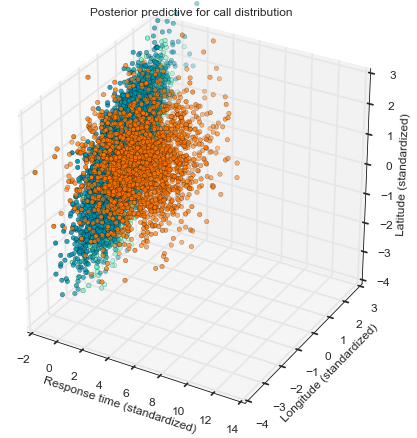
\includegraphics[width=45mm, height=42mm]{callposteriorpredictive}
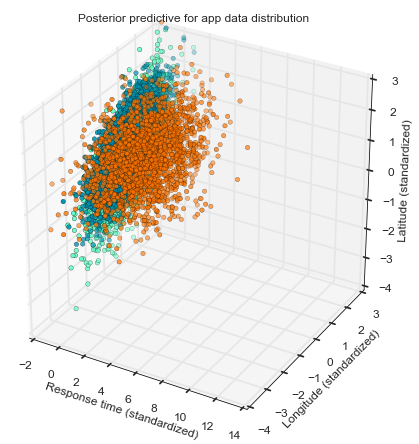
\includegraphics[width=45mm, height=42mm]{appposteriorpredictive}
\caption{Posterior predictive distributions}
\label{pred}
\end{center}
\end{figure}

\subsection{Posterior predictive}
To assess how well the model describes the data, we simulated data with the posterior predictive distribution. The posterior predictive distribution is generated by sampling from the posterior distribution obtained through Gibbs sampling, then using those parameter values to sample from the likelihood. The posterior predictive distributions for the app and call data are shown in Figure \ref{pred}. The posterior predictive distribution suggests that the choice of a Gaussian mixture model partly reflects the composition of the observations, tightly grouped components at lower response times and a more diffuse, lagging component with larger response times. The geographic difference between Citizens Connect and call data is also partially captured, with the posterior predictive distribution of the app data resulting in more compact components that are shifted to the northeast, which reflects the more typical geographic range of the app users. Gaussians are a reasonable first approximation for capturing the shape of the region over which the requests originate, since the latitude and longitudes of the requests are spread fairly symmetrically. However, a better model is needed to fit for the very longest response times. Given that our models found that clustering tended to occur along the response time axis, an alternative modeling approach would be to model response time as a one-dimensional problem. We explored posterior predictive distributions of single exponential and two-component exponential mixture models for the app data response times and found that the exponential mixture model was more consistent with the data compared to a single exponential (Figure \ref{expo}). This alternative suggests that requests can be described robustly as distinct populations of fast and lagging response times even under different modeling approaches. 

\begin{figure}[h!]
\begin{center}
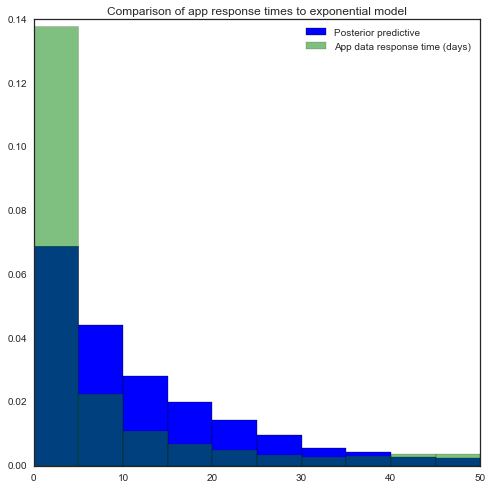
\includegraphics[width=45mm, height=42mm]{expomodel}
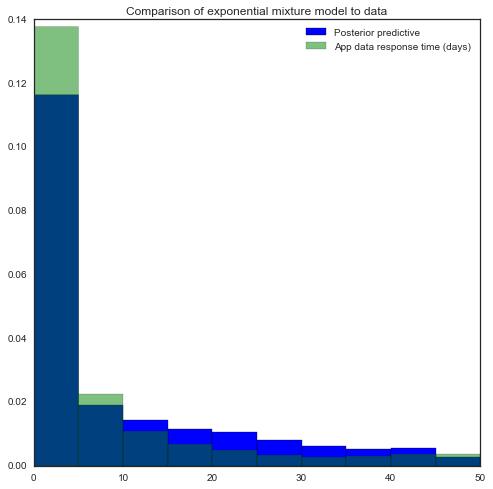
\includegraphics[width=45mm, height=42mm]{mixture}
\caption{Posterior predictive distributions for exponential and exponential mixture modeling of app response times only}
\label{expo}
\end{center}
\end{figure}


\section{Conclusion}
While the estimated means and covariances of the components of the model show some sensitivity to choice of technique, the broad trend remains that the components in the data are largely distinguished by differences in mean response times rather than showing strong separation in both response time and geography. Based on this clustering pattern, it does not appear that specific regions of the city face disproportionately slow response times (although this could be true on regional scales smaller than what a 3-component model can probe). 

\begin{figure}
\begin{center} \label{profiles}
\caption{Department breakdown of clusters}
\subfigure[MAP Clustering (Call Data)]{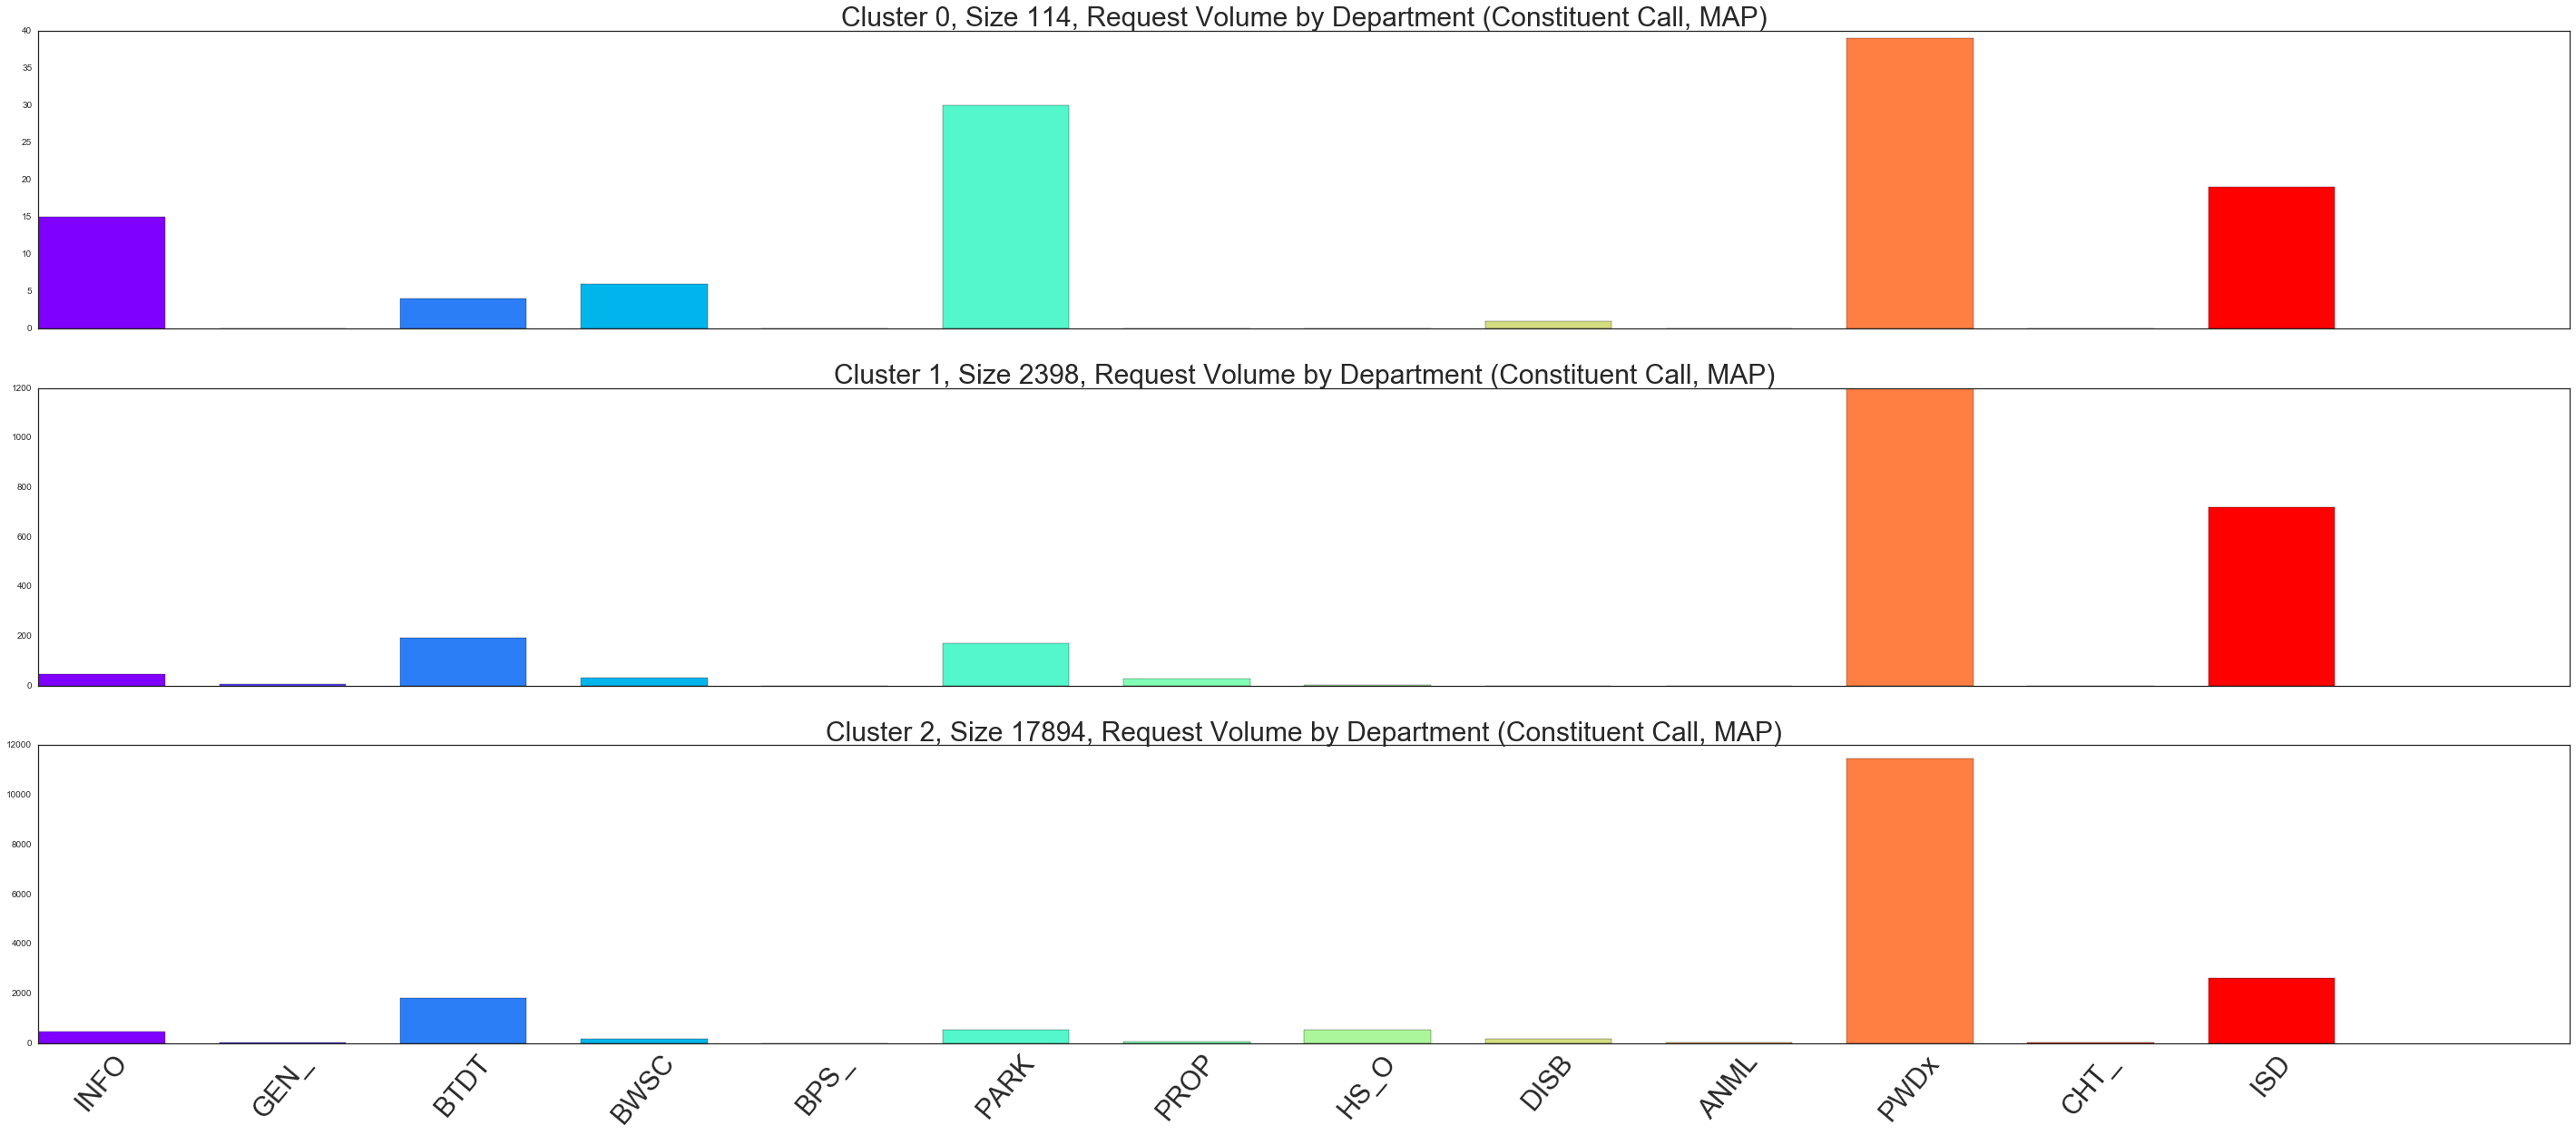
\includegraphics[height=38mm]{profile_call}}{} %height=30mm
\hskip1cm
\subfigure[MAP Clustering (App Data)]{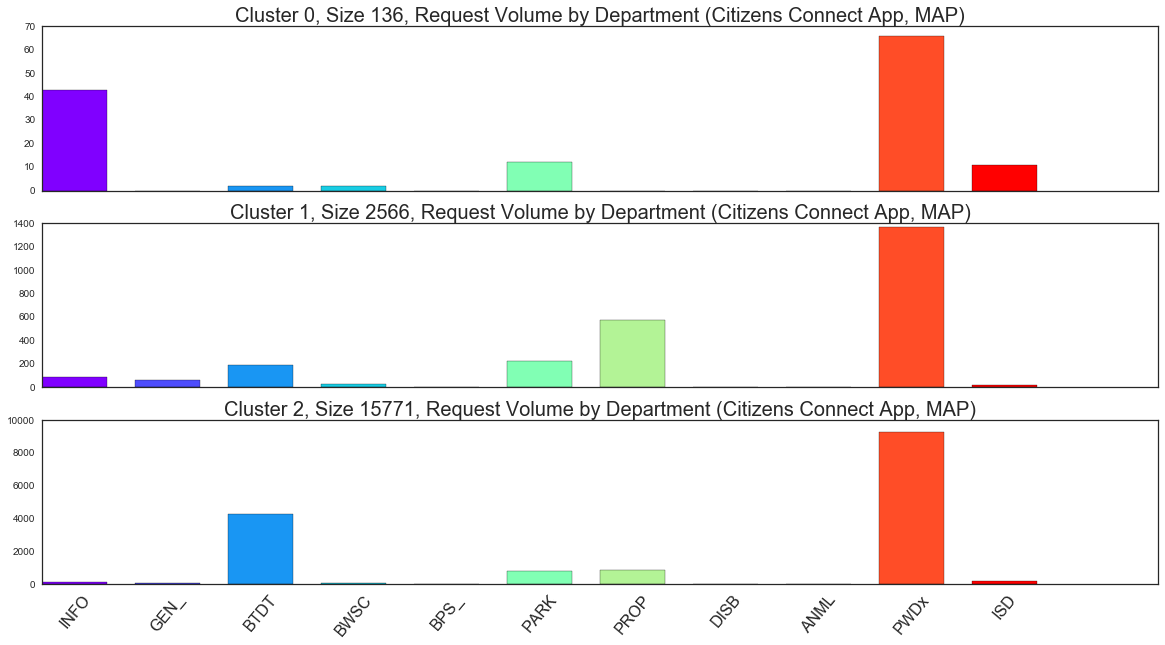
\includegraphics[height=38mm]{profile_app}}
\end{center}
\vskip -0.2in
\end{figure} 

To determine what characteristics may distinguish the different clusters of requests identified by the model (using the MAP assignments), we retrieved the distribution of requests by department in each cluster. The department volume profiles shown in Figure 9 indicate that for a given request type (eg., call or app), different departments become more prominent for components associated with different response times, which could suggest that the separation of requests into different components is attributable to different service need profiles. On the other hand, even though both Citizens Connect and constituent call data have components that are similarly oriented with respect to response time, their department volume profiles differ. This suggests that the characteristic lagging component observed for each group is not a straightforward matter of the same departments systematically taking longer.  Overall, our results suggest that while Citizens Connect and constituent calls tend toward different service needs and geographical origins, users of the app can expect responses similarly efficient to those received by 311 callers.


\bibliographystyle{abbrv}
\bibliography{GMMBib}

\end{document}





